
%(BEGIN_QUESTION)
% Copyright 2009, Tony R. Kuphaldt, released under the Creative Commons Attribution License (v 1.0)
% This means you may do almost anything with this work of mine, so long as you give me proper credit

In this process, maple syrup is heated as it passes through a steam heat exchanger, then enters an evaporator where the water boils off.  The purpose of this is to raise the sugar concentration of the syrup, making it suitable for use as a food topping.  A level control system (LT, LIC, and LV) maintains constant syrup level inside the evaporator, while an analytical control system (AT, AIR, AC, and AV) monitors the sugar concentration of the syrup and adjusts steam flow to the heat exchanger accordingly.

$$\includegraphics[width=15.5cm]{i04389x01.eps}$$

Suppose the level control valve (LV) fails completely open.  Determine the effect this failure will have on the sugar concentration of the outgoing syrup.

\vskip 20pt \vbox{\hrule \hbox{\strut \vrule{} {\bf Suggestions for Socratic discussion} \vrule} \hrule}

\begin{itemize}
\item{} Identify a few realistic reasons why the level control valve might fail all the way open in a process such as this.
\item{} Suppose the compressor speed is suddenly reduced.  What effect will this have on the control systems in this process, as well as syrup quality?
\end{itemize}

\underbar{file i04389}
%(END_QUESTION)





%(BEGIN_ANSWER)

%(END_ANSWER)





%(BEGIN_NOTES)

Since there will no longer be a retention time for syrup in the evaporator, less water will evaporate from the heated syrup, resulting in a more ``watery'' (less concentrated) syrup exiting the evaporator.

%INDEX% Basics, control loop troubleshooting: determining effect of specified fault(s)
%INDEX% Process: maple syrup concentration (single-effect evaporator)

%(END_NOTES)


